\setcounter{equation}{0}

\chapter{Introduction}

\noindent The rapid advancement of Artificial Intelligence (AI)\nomenclature{AI}{Artificial Intelligence} has revolutionized various aspects of human workflow, particularly in the field of data processing. One prominent application is the automation of handwritten digit recognition, which holds immense potential for numerous purposes. While recognizing digits from a small set can be relatively straightforward, dealing with vast quantities of handwritten digits poses significant challenges, as
it becomes a time-consuming task prone to errors.

\noindent To address this pressing challenge, the project aims to develop a robust and reliable system capable of instantaneously converting handwritten digits into structured Comma Separated Values(CSV)\nomenclature{CSV}{Comma Separated Values} files. By doing so, it alleviates the substantial burden placed on educators during the manual data entry process. This innovative system will empower teachers and researchers to allocate their valuable time more efficiently towards other essential responsibilities, ultimately enhancing the efficiency and accuracy of digit data processing in various domains.

\begin{figure}[h!]
    \centering
{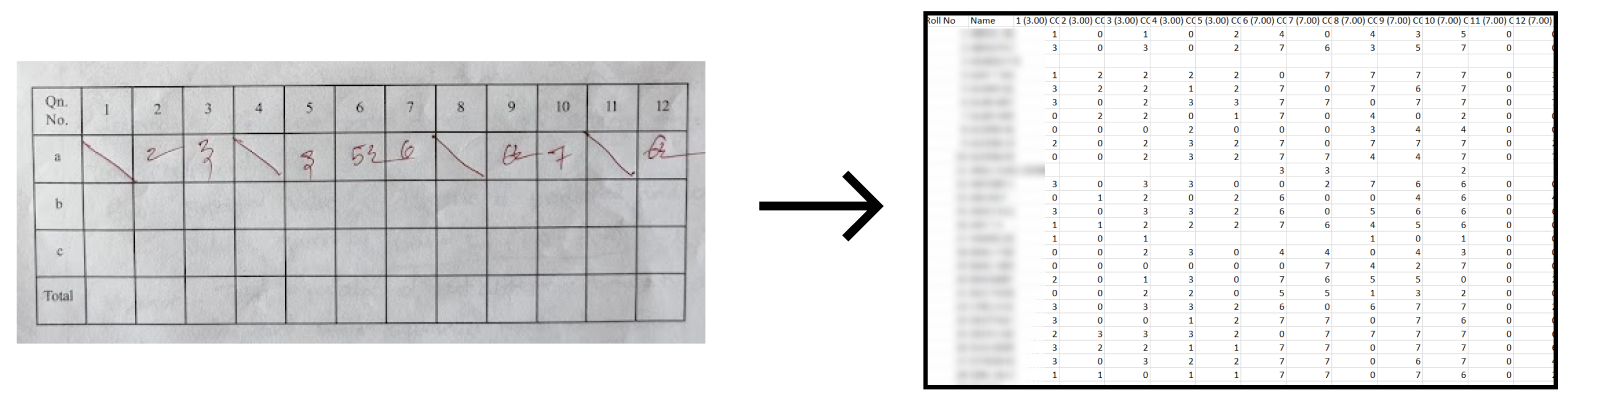
\includegraphics[width=0.9\textwidth]{Images/Intro/intro_pic.jpg}}
  \caption{Handwritten Text to Digital Text}
\end{figure}

\clearpage

\section{Background}

\noindent In modern education, the digitalization of student exam scores and data is not only crucial for administrative and academic purposes but also a transformative necessity for educational institutions. As the volume of student data grows exponentially, manual data entry becomes increasingly cumbersome and error-prone, leading to inefficiencies and potential inaccuracies in record-keeping. This highlights the urgent need for automated solutions that can handle this task efficiently and accurately.

\noindent Computer software, especially powered by AI and machine learning, plays a pivotal role in addressing these challenges and revolutionizing the education sector by the extraction and conversion of handwritten exam scores into standardized formats like Comma Separated Values (CSV) files. This automation not only saves valuable time and effort for educators but also drastically reduces the risk of transcription errors, ensuring the integrity of student records.

\noindent Furthermore, the benefits of digitalization extend far beyond administrative ease. With computer software handling data processing, teachers can dedicate more time and attention to enhancing the learning experience for students. By gaining insights from the digitized data, educators can identify areas of improvement, tailor teaching approaches to meet individual student needs and implement targeted interventions to support struggling learners.

\noindent Standardization through CSV files empowers educational institutions with organized and easily accessible data, enabling sophisticated data management and analysis. It equips educators and administrators with actionable insights into student performance trends, curriculum effectiveness, and overall institutional performance. Armed with this knowledge, institutions can make data-driven decisions, optimize educational practices, and design evidence-based interventions to maximize student outcomes.

\clearpage

\section{Motivation}

\noindent The primary focus of this project is to overcome the existing challenges that teachers encounter while digitizing student exam scores. The traditional method of manually entering data into spreadsheets or databases is a time-consuming and error-prone process. By utilizing the power of AI and machine learning, the project aims to create an automated system that can efficiently and accurately extract relevant data from answer scripts and convert it into standardized CSV files.


\noindent A key motivation for this project is to relieve educators from the burdening task of manual data entry. By freeing up the valuable time of teachers, they can redirect their efforts toward more critical aspects of their profession. For example, teachers can focus on creating engaging and effective lesson plans suitable to the needs of their students. Additionally, with more time at hand, teachers can offer personalized support to students, providing them with the attention and assistance they require to excel in their studies. Moreover, the automation of data conversion empowers teachers to invest in their own professional development. They can use the saved time to attend workshops, engage in research, collaborate with colleagues, and explore innovative teaching methodologies. This, in turn, enhances their teaching skills.

\noindent Furthermore, the automated system brings about operational efficiency within educational institutions. By reducing the reliance on manual data entry, the risk of transcription errors is minimized, ensuring the accuracy and integrity of student records. The availability of reliable data enables educational institutions to make informed decisions, assess student performance, and identify areas of improvement in the curriculum.
\clearpage

\section{Objective and Scope}

\subsection{Objective}

The objective of this project is to develop a tool to assist teachers in the data entry process by implementing an efficient Optical Character Recognition (OCR)\nomenclature{OCR}{Optical Character Recognition} system using the Convolutional Neural Network (CNN)\nomenclature{CNN}{Convolutional Neural Network} architecture. The tool aims to streamline the extraction of table marks from various images, enhancing accuracy and reducing manual effort. By utilizing the power of OCR technology, the tool will automate the recognition and extraction of digits from images which save teachers valuable time and minimize errors. Furthermore, the customizable nature of the program will enable programmers to define their specific parameters and rules for extracting marks as per institutional requirements. Ultimately, this project aims to provide teachers with a reliable and efficient solution for data entry, optimizing their productivity and facilitating their administrative tasks.

\subsection{Scope}

In recent years, the rapid development of AI has witnessed remarkable advancements, particularly in the domain of computer vision and optical character recognition (OCR). These developments become a stepping stone for innovative applications in various sectors, including education. The scope of this project aligns perfectly with these recent AI developments, as it aims to leverage cutting-edge neural networks to automate the conversion of images of answer scripts into CSV format.

\noindent The utilization of neural networks for digit classification is a key highlight of this project. Neural networks have demonstrated very high accuracy in recognizing and classifying complex patterns, such as handwritten digits. By utilizing this technology, the automated system can achieve high precision in identifying and extracting numerical scores from answer scripts. Additionally, the system will be designed to detect decimal marks during the OCR processing stage.

\clearpage

\noindent As a result, the automated system becomes adaptable to a wide range of educational institutions and their specific scoring requirements, offering customers the flexibility of customization in mark detection. Furthermore, a compact and portable device will be created to encapsulate the tool, enhancing usability and convenience. Advancements in microprocessors and other techniques will help to design powerful AI-driven devices that are small, lightweight, and highly portable this portable solution promises to facilitate the digitization of scores and streamline the grading process, saving time and effort for educators while providing valuable insights into student performance.

\section{Contributions}

\noindent The primary contribution to this system involved extensive research and development efforts in creating a novel Convolutional Neural Network (CNN) model entirely from scratch. This undertaking required in-depth knowledge of deep learning architectures and image processing techniques.

\noindent The newly developed CNN model was carefully integrated into the proposed system, which was designed to address a specific problem or task. Once the model was fully implemented, a comprehensive evaluation process was conducted to assess its performance and capabilities.

\noindent To gauge the effectiveness of the proposed system, a comparison was made between the performance metrics of the newly developed model and those of other existing systems that were considered state-of-the-art in the field. This comparison was conducted using standardized evaluation metrics, ensuring a fair and objective assessment.

\noindent The results of this comparative analysis revealed a significant difference in efficiency, with the proposed system showcasing superior performance compared to the existing alternatives. The newly developed CNN model demonstrated higher accuracy, faster processing speed and other relevant improvements on the specific task at hand. The observed superiority of the proposed system over other existing solutions is a clear testament to the effectiveness of the new CNN model and its successful integration into the overall system architecture.